%%%%%%%%%%%%%%%%%%%%%%%%%%%%%%%%%%%%%%%%%%%%%%%%%%%%%%%%%%%%%%%%%%%%%%%%%%%%%%%
\documentclass[hyperref={pdfpagelabels=false},compress,table]{beamer} % 在Mac下无法编译
% \documentclass[compress,table]{beamer} % 在Mac下使用
% package for font
\usepackage{fontspec}
\defaultfontfeatures{Mapping=tex-text}  %%如果没有它,会有一些 tex 特殊字符无法正常使用,比如连字符。
\usepackage{xunicode,xltxtra}
\usepackage[BoldFont,SlantFont,CJKnumber,CJKchecksingle]{xeCJK}  % \CJKnumber{12345}: 一万二千三百四十五
\usepackage{CJKfntef}  %%实现对汉字加点、下划线等。
\usepackage{pifont}  % \ding{}
% package for math
\usepackage{amsfonts}

% package for graphics
\usepackage[americaninductors,europeanresistors]{circuitikz}
\usepackage{tikz}
\usetikzlibrary{plotmarks}  % placements=positioning
\usepackage{graphicx}  % \includegraphics[]{}
\usepackage{subfigure}  %%图形或表格并排排列
% package for table
\usepackage{colortbl,dcolumn}  %% 彩色表格
\usepackage{multirow}
\usepackage{multicol}
\usepackage{booktabs}
% package for code
\usepackage{fancyvrb}
\usepackage{listings}

% \usepackage{animate}
% \usepackage{movie15}

%%%%%
% setting for beamer
\usetheme{default} % Madrid(常用), Copenhagen, AnnArbor, boxes(白色), Frankfurt,Berkeley
\useoutertheme[subsection=true]{miniframes} % 使用Berkeley时注释本行
\usecolortheme{sidebartab}
\usefonttheme{serif}  %%英文使用衬线字体
% \setbeamertemplate{background canvas}[vertical
% shading][bottom=white,top=structure.fg!7] %%背景色,上25%的蓝,过渡到下白。
\setbeamertemplate{theorems}[numbered]
\setbeamertemplate{navigation symbols}{}  %% 去掉页面下方默认的导航条
\setbeamercovered{transparent}  %设置 beamer 覆盖效果

% 设置标题title背景色
% \setbeamercolor{title}{fg=black, bg=lightgray!60!white}
\setbeamercolor{title}{fg=white, bg=black!70!white}

% 设置每页小LOGO
\pgfdeclareimage[width=1cm]{ouc}{figures/static/ouc.pdf}
\logo{\pgfuseimage{ouc}{\vspace{-20pt}}}

% setting for font
%%\setCJKmainfont{Adobe Kaiti Std}
\setCJKmainfont{SimSun} 
%% \setCJKmainfont{FangSong_GB2312} 
%% \setmainfont{Apple Garamond}  %%苹果字体没有SmallCaps
\setCJKmainfont{SimSun} 
%FUNNY%\setCJKmainfont{DFPShaoNvW5-GB}  %%华康少女文字W5(P)
%FUNNY%\setCJKmainfont{FZJingLeiS-R-GB}  %%方正静蕾体
%FUNNY%\setmainfont{Purisa}
%\setsansfont[Mapping=tex-text]{Adobe Song Std}
     %如果装了Adobe Acrobat,可在font.conf中配置Adobe字体的路径以使用其中文字体。
     %也可直接使用系统中的中文字体如SimSun、SimHei、微软雅黑等。
     %原来beamer用的字体是sans family;注意Mapping的大小写,不能写错。
     %设置字体时也可以直接用字体名,以下三种方式等同:
     %\setromanfont[BoldFont={黑体}]{宋体}
     %\setromanfont[BoldFont={SimHei}]{SimSun}
     %\setromanfont[BoldFont={"[simhei.ttf]"}]{"[simsun.ttc]"}
% setting for graphics
\graphicspath{{figures/}}  %%图片路径
\renewcommand\figurename{图}

% setting for pdf
\hypersetup{% pdfpagemode=FullScreen,%
            pdfauthor={Xiaodong Wang},%
            pdftitle={Title},%
            CJKbookmarks=true,%
            bookmarksnumbered=true,%
            bookmarksopen=false,%
            plainpages=false,%
            colorlinks=true,%
            citecolor=green,%
            filecolor=magenta,%
            linkcolor=blue,%red(default)
            urlcolor=cyan}

% setting for fontspec
\XeTeXlinebreaklocale "zh"  %%表示用中文的断行
\XeTeXlinebreakskip = 0pt plus 1pt minus 0.1pt  %%多一点调整的空间
%%%%%

% font setting by xeCJK
\setCJKfamilyfont{NSimSun}{NSimSun}
\newcommand{\song}{\CJKfamily{NSimSun}}
%%%\setCJKfamilyfont{AdobeSongStd}{Adobe Song Std}
%%%\newcommand{\AdobeSong}{\CJKfamily{AdobeSongStd}}
\setCJKfamilyfont{FangSong}{FangSong_GB2312}
\newcommand{\fang}{\CJKfamily{FangSong}}
%%%\setCJKfamilyfont{AdobeFangsongStd}{Adobe Fangsong Std}
%%%\newcommand{\AdobeFang}{\CJKfamily{AdobeFangsongStd}}
\setCJKfamilyfont{SimHei}{SimHei}
\newcommand{\hei}{\CJKfamily{SimHei}}
%%%\setCJKfamilyfont{AdobeHeitiStd}{Adobe Heiti Std}
%%%\newcommand{\AdobeHei}{\CJKfamily{AdobeHeitiStd}}
\setCJKfamilyfont{KaiTi}{KaiTi}
\newcommand{\kai}{\CJKfamily{KaiTi}}
%%%\setCJKfamilyfont{AdobeKaitiStd}{Adobe Kaiti Std}
\newcommand{\AdobeKai}{\CJKfamily{AdobeKaitiStd}}
\setCJKfamilyfont{LiSu}{LiSu}
\newcommand{\li}{\CJKfamily{LiSu}}
\setCJKfamilyfont{YouYuan}{YouYuan}
\newcommand{\you}{\CJKfamily{YouYuan}}
\setCJKfamilyfont{FZJingLei}{FZJingLeiS-R-GB}
\newcommand{\jinglei}{\CJKfamily{FZJingLei}}
\setCJKfamilyfont{MSYH}{Microsoft YaHei}
\newcommand{\msyh}{\CJKfamily{MSYH}}

% 自定义颜色
\def\Red{\color{red}}
\def\Green{\color{green}}
\def\Blue{\color{blue}}
\def\Mage{\color{magenta}}
\def\Cyan{\color{cyan}}
\def\Brown{\color{brown}}
\def\White{\color{white}}
\def\Black{\color{black}}

\lstnewenvironment{xmlCode}[1][]{% for Java
  \lstset{
    basicstyle=\tiny\ttfamily,%
    columns=flexible,%
    framexleftmargin=.7mm, %
    % frame=shadowbox,%
    % rulesepcolor=\color{cyan},%
     frame=single,%
    backgroundcolor=\color{white},%
    xleftmargin=4\fboxsep,%
    xrightmargin=4\fboxsep,%
    numbers=left,numberstyle=\tiny,%
    numberblanklines=false,numbersep=7pt,%
    language=xml, %
    }\lstset{#1}}{}

\lstnewenvironment{javaCode}[1][]{% for Java
  \lstset{
    basicstyle=\tiny\ttfamily,%
    columns=flexible,%
    framexleftmargin=.7mm, %
    frame=shadowbox,%
    rulesepcolor=\color{cyan},%
    % frame=single,%
    backgroundcolor=\color{white},%
    xleftmargin=4\fboxsep,%
    xrightmargin=4\fboxsep,%
    numbers=left,numberstyle=\tiny,%
    numberblanklines=false,numbersep=7pt,%
    language=Java, %
    }\lstset{#1}}{}

\lstnewenvironment{shCode}[1][]{% for Java
  \lstset{
    basicstyle=\scriptsize\ttfamily,%
    columns=flexible,%
    framexleftmargin=.7mm, %
    frame=shadowbox,%
    rulesepcolor=\color{brown},%
    % frame=single,%
    backgroundcolor=\color{white},%
    xleftmargin=4\fboxsep,%
    xrightmargin=4\fboxsep,%
    numbers=left,numberstyle=\tiny,%
    numberblanklines=false,numbersep=7pt,%
    language=sh, %
    }\lstset{#1}}{}

\newcommand\ask[1]{\vskip 4bp \tikz \node[rectangle,rounded corners,minimum size=6mm,
  fill=white,]{\Cyan \includegraphics[height=1.5cm]{question} \Large \msyh #1};}

\newcommand\wxd[1]{\vskip 4bp \tikz \node[rectangle,minimum size=6mm,
  fill=blue!60!white,]{\White \ding{118} \msyh #1};}

\newcommand\xyy[1]{\vskip 2bp \tikz \node[rectangle,minimum size=3mm,
  fill=black!80!white,]{\White \msyh\scriptsize #1};}

\newcommand\cxf[1]{\vskip 4bp \tikz \node[rectangle,rounded corners,minimum size=6mm,
  fill=orange!60!white,]{\White \ding{42} \msyh #1};}

\newcommand\samp[1]{\vskip 2bp \tikz \node[rectangle,minimum size=3mm,
  fill=white!100!white,]{\Mage\msyh \small CODE \ding{231} \Black #1};\vskip -8bp}

\newcommand\zhyfly[1]{\tikz \node[rectangle,rounded corners,minimum size=6mm,ball color=red!25!blue,text=white,]{#1};}

\setbeamerfont{frametitle}{series=\msyh} % 修改Beamer标题字体

\makeatletter
\newcommand{\Extend}[5]{\ext@arrow 0099{\arrowfill@#1#2#3}{#4}{#5}}
\makeatother


%%%%%%%%%%%%%%%%%%%%%%%%%%%%%%%%%%%%%%%%%%%%%%%%%%%%%%%%%%%%%%%%%%%%%%%%%%%%%%%
% \titlepage
\title[KevinW@OUC]{\hei {\huge Java 应用与开发}\\  
  线程编程}
\author[王晓东]{王晓东\\
  \href{mailto:wangxiaodong@ouc.edu.cn}{\footnotesize wangxiaodong@ouc.edu.cn}}
\institute[中国海洋大学]{\small 中国海洋大学}
\date{\today}
\titlegraphic{\vspace{-6em}
\includegraphics[height=6cm]{static/ouc.pdf}\vspace{-6em}}
%%%%%
\begin{document}
%% Delete this, if you do not want the table of contents to pop up at
%% the beginning of each subsection:
\AtBeginSection[]{                              % 在每个Section前都会加入的Frame
  \frame<handout:0>{
    \frametitle{\textbf{\hei 接下来…}}
    \tableofcontents[currentsection]
  }
}  %

\AtBeginSubsection[]                            % 在每个子段落之前
{
  \frame<handout:0>                             % handout:0 表示只在手稿中出现
  {
    \frametitle{\textit{\hei 接下来…}}\small
    \tableofcontents[current,currentsubsection] % 显示在目录中加亮的当前章节
  }
}
\frame{\titlepage}
%%%%%%%%%%%%%%%%%%%%%%%%%%%%%%%%%%%%%%%%%%%%%%%%%%%%%%%%%%%%%%%%%%%%%%%%%%%%%%%
\begin{frame}
  \frametitle{学习目标}
  \begin{enumerate}
  \item 线程基础
  \item 线程控制
  \item 线程的同步
  \end{enumerate}  
\end{frame}

\section*{大纲}
\frame{\frametitle{大纲} \tableofcontents }
%%%%%%%%%%%%%%%%%%%%%%%%%%%%%%%%%%%%%%%%%%%%%%%%%%%%%%%%%%%%%%%%%%%%%%%%%%%%%%%

\section{线程基础}
% \subsection{线程的概念模型}

\begin{frame}[fragile]
  \frametitle{概念回顾}

  \tta{任务调度}
  
  \begin{itemize}
  \item 大部分操作系统的任务调度是采用{\hei\Red 时间片轮转的抢占式调度方式},一个
    任务执行一小段时间后强制暂停去执行下一个任务,每个任务轮流执行。
  \item CPU的执行效率非常高,时间片非常短,在各个任务之间快速地切换,让
    人感觉像是多个任务在“同时进行”,这也就是我们所说的{\hei\Red 并发}。
  \end{itemize}

  \begin{figure}
    \centering
    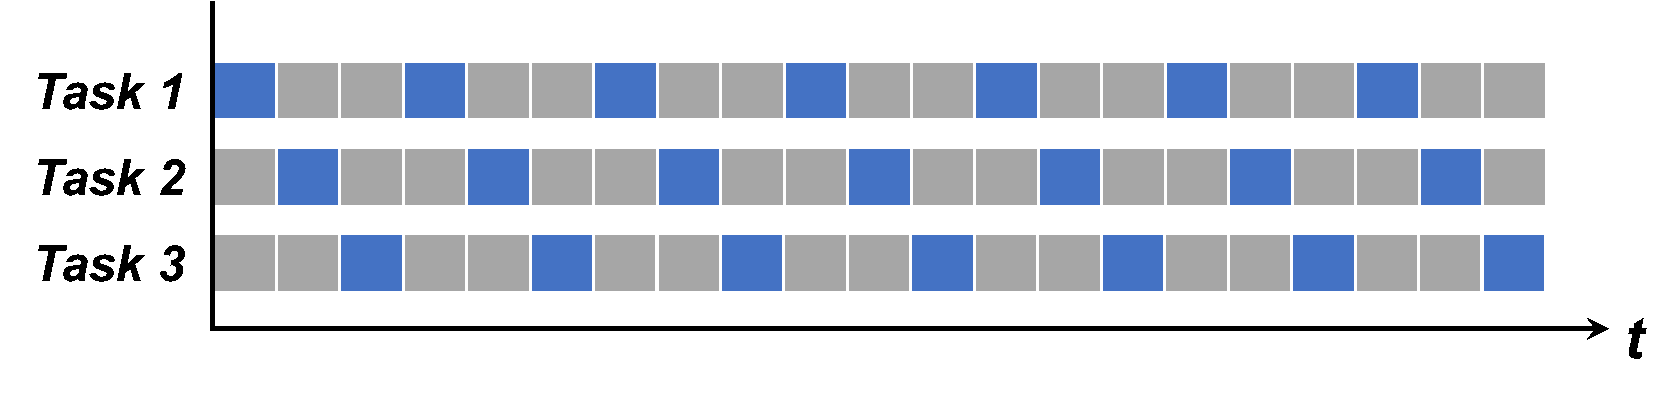
\includegraphics[width=0.9\textwidth]{time-split.pdf}
  \end{figure}
\end{frame}

\begin{frame}[fragile]
  \frametitle{概念回顾}

  \tta{进程}
  
  \begin{itemize}
  \item 进程是一个具有一定独立功能的程序在一个数据集上的一次动态执行的
    过程,是操作系统进行资源分配和调度的一个独立单位,是应用程序运行的
    载体。

    {\kai\Red (展示类UNIX系统的进程树)}
    
  \item 进程一般由{\hei\Blue 程序段、数据段和进程控制块}三部分构成进程实体。
  \end{itemize}
\end{frame}


\begin{frame}[fragile] % [fragile]参数使得能够插入代码
  \frametitle{什么是线程}

  根据多任务原理,在一个程序内部也可以实现多个任务(顺序控制流)的并发执行,其中每个任务被
  称为{\hei\Red 线程(Thread)}。更专业的表述为:

  {\Blue\hei 线程是程序内部的顺序控制流。}
\end{frame}

\begin{frame}[fragile] % [fragile]参数使得能够插入代码
  \frametitle{线程和进程的区别和联系}

  \begin{figure}
    \centering
    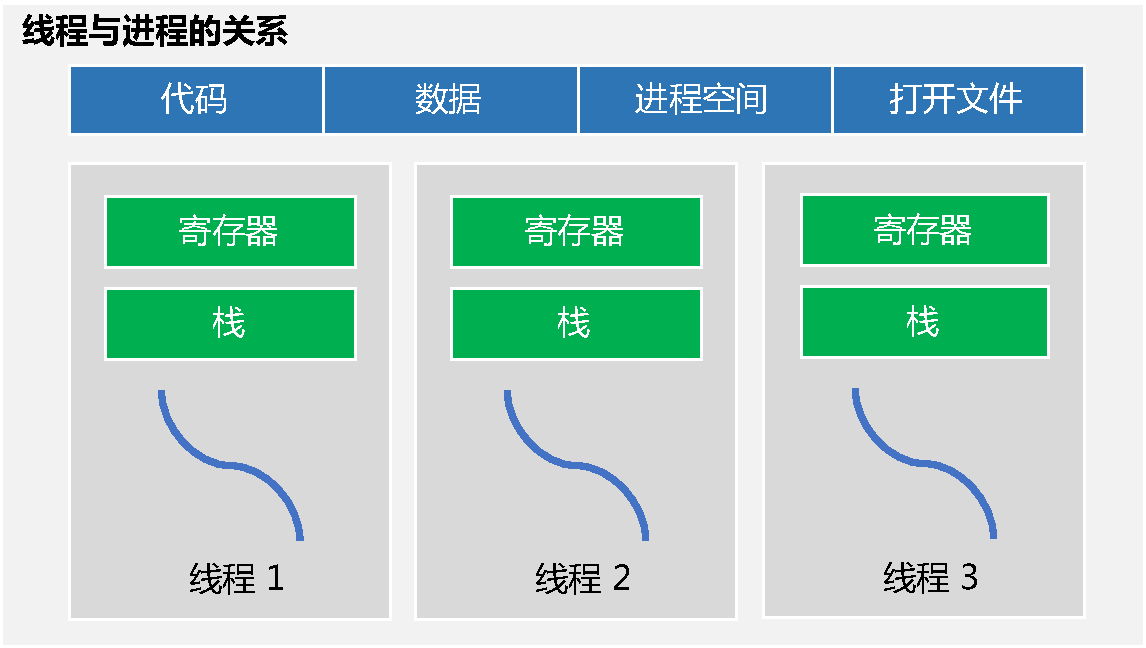
\includegraphics[width=0.6\textwidth]{threads-within-process.pdf}
  \end{figure}
  \pause
  \begin{enumerate}\small\kai
  \item 每个进程都有独立的代码和数据空间(进程上下文),进程切换的开销大。
  \item 线程作为“轻量的进程”,同一类线程共享代码和数据空间,每个线程有独立
    的运行栈和程序计数器(PC),线程切换的开销小。
  \item 多进程——在操作系统中能同时运行多个任务(程序)。
  \item 多线程——在同一应用程序中有多个顺序流同时执行。
  \end{enumerate}
\end{frame}

\begin{frame}[fragile]
  \frametitle{多核与多线程}
  \begin{itemize}
  \item 多核处理器是指在一个处理器上集成多个运算核心以提高并行计算能力,
    每一个处理核心对应一个内核线程(Kernel Thread, KLT)。
  \item 内核线程是直接由操作系统内核支持的线程,由内核来完成线程切换,
    内核通过操作调度器对线程进行调度,并负责将线程的任务映射到各个处理
    器上。
  \end{itemize}

  %% https://blog.csdn.net/luoweifu/article/details/46595285
\end{frame}

\begin{frame}[fragile]
  \frametitle{多核与多线程}
  一般一个处理核心对应一个内核线程,比如单核处理器对应一个内核线程,双
  核处理器对应两个内核线程。

  {\Red\kai 而现代计算机采用超线程技术将一个物理处理核心模拟成两个逻辑
    处理核心对应两个内核线程,一般是双核四线程、四核八线
    程。\footnote{课后自行搜索了解超线程的概念,内核线程与用户线程的映
      射}}

  \begin{figure}
\centering
\fbox{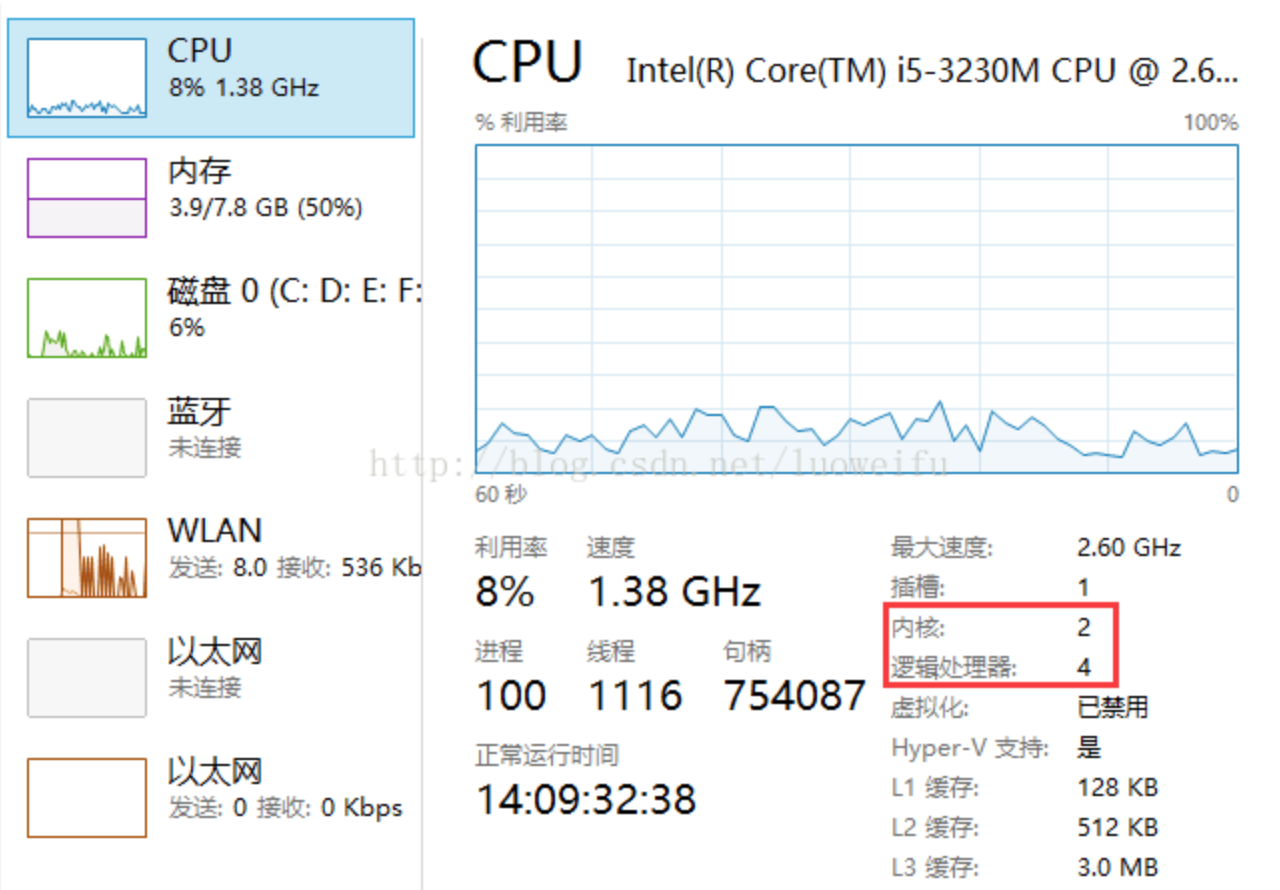
\includegraphics[width=0.5\textwidth]{multi-cores-and-threads.png}}
\end{figure}
\end{frame}

\begin{frame}[fragile] % [fragile]参数使得能够插入代码
\frametitle{Java线程的概念模型}

在Java语言中,多线程的机制通过{\hei 虚拟CPU}来实现。

\begin{enumerate}\kai
\item 虚拟的CPU,由java.lang.Thread类封装和虚拟;
\item CPU所执行的代码和数据,传递给Thread类对象。
\end{enumerate}
\begin{figure}
\centering
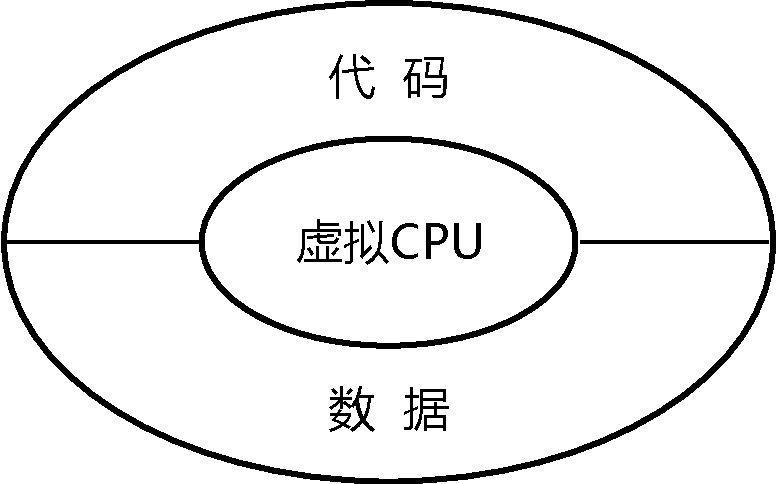
\includegraphics[width=0.5\textwidth]{virtual-cpu.pdf}
\end{figure}
\end{frame}

% \subsection{创建线程}

\begin{frame}[fragile] % [fragile]参数使得能够插入代码
  \frametitle{创建和启动线程的一般步骤}

  每个线程都是通过某个特定Thread对象所对应的方法run()来完成其操作,方
  法run()称为{\hei\Red 线程体}。
  
  \begin{enumerate}[<+-| alert@+>]\kai
  \item 定义一个类实现Runable接口,重写其中的run()方法,加入所需的处理逻辑;
  \item 创建Runable接口实现类的对象;
  \item 创建Thread类的对象(封装Runable接口实现类型对象);
  \item 调用Thread对象的start()方法,启动线程。
  \end{enumerate}

  \codeset{sample.thread.FirstThreadSample.java}
\end{frame}

\begin{frame}[fragile] % [fragile]参数使得能够插入代码
  \frametitle{多线程}

  Java中引入线程机制的目的在于实现{\hei\Red 多线程(Multi-Thread)并发执
    行,以及实现多任务之间的协同}。

  \tta{使用多线程}

  \codeset{sample.thread.MultiThreadsSample.java}
\end{frame}

\begin{frame}[fragile] % [fragile]参数使得能够插入代码
  \frametitle{多线程}

  \tta{多线程之间可以共享代码和数据}

  \begin{javaCode}
    Runner2 r = new Runner2();
    Thread t1 = new Thread(r);
    Thread t2 = new Thread(r);
  \end{javaCode}
  \begin{table}
    \footnotesize
    \setlength{\extrarowheight}{1.2mm}
    \rowcolors[]{1}{blue!20}{blue!10}
    \begin{tabular}{c|c|c}
      {\bf 线程} & {\bf 虚拟CPU} & {\bf 代码} \\
      t1 & Thread类对象 & Runner2类中的run()方法 \\
      t2 & Thread类对象 & Runner2类中的run()方法 \\
    \end{tabular}
  \end{table}
\end{frame}

\begin{frame}[fragile] % [fragile]参数使得能够插入代码
  \frametitle{创建线程的第二种方式}

  \ttc{直接继承Thread类创建线程}
  \begin{javaCode}
    public class TestThread3 {
      public static void main(String args[]) {
        Thread t = new Runner3();
        t.start();
      }
    }
    class Runner3 extends Thread {
      public void run() {
        for(int i=0; i<30; i++) {
          System.out.println("No. " + i);
        }
      }
    }
  \end{javaCode}

  \tta{第二种创建线程的方式}
  \begin{enumerate}
  \item 定义一个类继承Thread类,重写其中的run()方法,加入所需的处理逻辑;
  \item 创建该Thread类的对象;
  \item 调用该对象的start()方法。
  \end{enumerate}
\end{frame}

\begin{frame}[fragile] % [fragile]参数使得能够插入代码
  \frametitle{两种创建线程的方式比较}
  \tta{使用Runnable接口创建线程}
  \begin{itemize}
  \item 可以将虚拟CPU、代码和数据分开,形成清晰的模型;
  \item 线程体run()方法所在的类还可以从其他类继承一些有用的属性或方法;
  \item 有利于保持程序风格的一致性。
  \end{itemize}

  \pause
  
  \tta{直接继承Thread类创建线程}
  \begin{itemize}
  \item Thread子类无法再从其他类继承;
  \item 编写简单,run()方法的当前对象就是线程对象,可直接操纵。
  \end{itemize}
\end{frame}

% \subsection{后台线程}
\begin{frame}[fragile] % [fragile]参数使得能够插入代码
  \frametitle{后台线程}

  \tta{相关概念}\\
  \ttc{后台处理} 是指在分时处理或多任务系统中,当实时、会话式、高优先级或
  需迅速响应的计算机程序不再使用系统资源时,计算机去执行较低优先级程序的
  过程。批量处理、文件打印通常采取后台处理的形式。\pause

  \ttc{后台线程} 是指那些在后台运行的,为其他线程提供服务的功能,如JVM的
  垃圾回收线程等,后台线程也称为守护线程(Daemon Thread)。\pause

  \ttc{用户线程} 和后台线程相对应,其他完成用户任务的线程可称为“用户线
  程”。
\end{frame}

\begin{frame}[fragile] % [fragile]参数使得能够插入代码
  \frametitle{后台线程}

  \tta{Thread类与后台线程相关的方法}

  \begin{enumerate}\kai
  \item 测试当前线程是否为守护线程,如果是则返回true,否则返回false
    \begin{javaCode}
      public final boolean isDaemon()
    \end{javaCode}
  \item 将当前线程标记为守护线程或用户线程,本方法必须在启动线程前调用
    \begin{javaCode}
      public final void setDaemon(Boolean on)
    \end{javaCode}
  \end{enumerate}

  \codeset{sample.thread.DaemonThreadSample.java}
\end{frame}

% \subsection{GUI线程}
\begin{frame}[fragile] % [fragile]参数使得能够插入代码
  \frametitle{GUI线程}

  GUI程序运行过程中,系统会自动创建若干GUI线程,以提供GUI程序运行所需的功能,主要包括:

  \begin{enumerate}\kai
  \item 窗体显示和重绘;
  \item GUI事件处理;
  \item 关闭抽象窗口工具集等。
  \end{enumerate}
\end{frame}

\begin{frame}[fragile] % [fragile]参数使得能够插入代码
\frametitle{GUI线程}

\ttc{使用GUI线程示例}
\samp{GUIThreadSample.java: Part 1}
\begin{javaCode}
import java.awt.*;
import java.awt.event.*;

public class GUIThreadSample {
  public static void main(String[] args) throws Exception {
    Frame f = new Frame();
    Button b = new Button("Press Me");
    MyMonitor mm = new MyMonitor();
    b.addActionListener(mm);
    f.addWindowListener(mm);
    f.add(b, "Center");
    f.setSize(100, 60);
    f.setVisible(true);
    MyThreadViewer.view();
  }
}
class MyMonitor extends WindowAdapter implements ActionListener {
  public void actionPerformed(ActionEvent e) {
    MyThreadViewer.view();
  }
}
\end{javaCode}
\end{frame}

\begin{frame}[fragile] % [fragile]参数使得能够插入代码
\frametitle{GUI线程}

\samp{GUIThreadSample.java: Part 2}
\begin{javaCode}
class MyThreadViewer {
  public static void view() {
    Thread current = Thread.currentThread();
    System.out.println("当前线程名称:" + current.getName());
    int total = Thread.activeCount();
    System.out.println("活动线程总数:" + total + "个");
    Thread[] threads = new Thread[total];
    current.enumerate(threads);
    for(Thread t: threads) {
      String role = t.isDaemon() ? "后台线程" : "用户线程";
      System.out.println("   -" + role + t.getName());
    }
    System.out.println("-------------------");
  }
}
\end{javaCode}
\end{frame}

%% \begin{frame}[fragile] % [fragile]参数使得能够插入代码
%% \frametitle{GUI线程}
%% 
%% \ttc{[API] Thread.enumerate}\\
%% Copies into the specified array every active thread in the current thread's thread group
%% and its subgroups. This method simply calls the enumerate method of the current thread's
%% thread group with the array argument.
%% 
%% First, if there is a security manager, that enumerate method calls the security
%% manager's checkAccess method with the thread group as its argument. This may result in
%% throwing a SecurityException.
%% 
%% Parameters: 
%% \begin{itemize}
%% \item tarray an array of Thread objects to copy to
%% \end{itemize}
%% Returns: 
%% \begin{itemize}
%% \item the number of threads put into the array
%% \end{itemize}
%% Throws:
%% \begin{itemize}
%% \item SecurityException - if a security manager exists and its checkAccess method
%%   doesn't allow the operation.
%% \end{itemize}
%% \end{frame}

\begin{frame}[fragile] % [fragile]参数使得能够插入代码
  \frametitle{GUI自动创建的线程}
  
\begin{itemize}[<+-| alert@+>]\kai
\item {\hei AWT-Windows线程}\\
  \only<1>{负责从操作系统获取底层事件通知,并将之发送到系统事件队列(EventQueue)等待处理。
    在其他平台上运行时,此线程的名字也会作相应变化,例如在Unix系统则为“AWT-Unix”。}
\item {\hei AWT-EventQueue-n线程}\\
  \only<2>{也称事件分派线程,该线程负责从事件队列中获取事件,将之分派到相应的GUI组件(事
    件源)上,进而触发各种GUI事件处理对象,并将之传递给相应的事件监听器进行处理。}
\item {\hei AWT-Shutdown线程}\\
\only<3>{负责关闭已启用的抽象窗口工具,释放其所占用的资源,该线程将等到其他GUI线程均退出
  后才开始其清理工作。}
\item {\hei DestroyJavaVM线程}\\
\only<4>{在所有其他用户线程退出后,负责释放任意线程所占用系统资源并卸载Java虚拟机。该线
  程在主线程运行结束时由系统自动启动,但要等到所有其他用户线程均退出后才开始其卸载工作。}
\end{itemize}
\end{frame}

\section{线程控制}
% \subsection{线程生命的周期}
\begin{frame}[fragile] % [fragile]参数使得能够插入代码
  \frametitle{线程的生命周期}
  
  \begin{description}[<+-| alert@+>]\kai
  \item[新建状态] 调用Thread构造方法,未显式调用start()方法前;
  \item[就绪状态] 调用start()方法后,线程在就绪队列里等候;
  \item[运行状态] 开始执行线程体代码;
  \item[阻塞状态] 因某事件发生,例如线程进行I/O操作,等待用户输入数据;
  \item[终止状态] 线程run()方法执行完毕。
  \end{description}

\begin{figure}
\centering
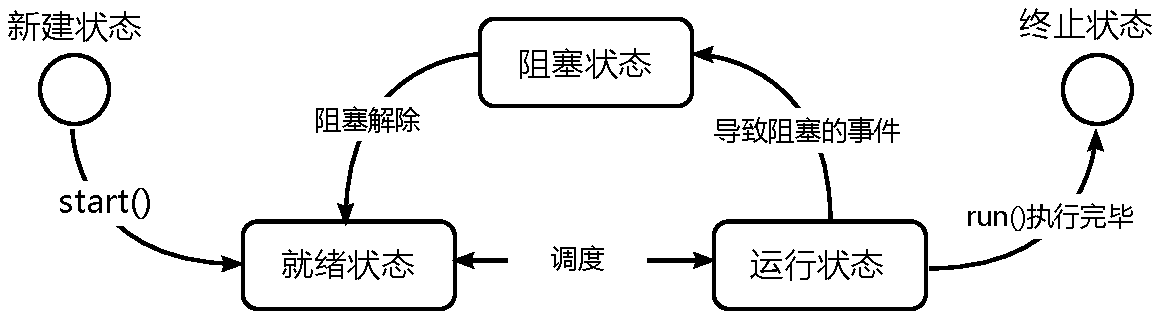
\includegraphics[width=0.7\textwidth]{fig02.pdf}
\end{figure}
\end{frame}

% \subsection{线程优先级}
\begin{frame}[fragile] % [fragile]参数使得能够插入代码
\frametitle{线程优先级}

线程的优先级用数字来表示,范围从1到10。主线程的缺省优先级是5,子线程的优先级默认与其父线
程相同。可以使用Thread类提供的方法获得和设置线程的优先级:

\begin{itemize}\kai
\item 获取当前线程优先级
  \begin{javaCode}
    public final int getPriority();
  \end{javaCode}
\item 设定当前线程优先级
  \begin{javaCode}
    public final void setPriority(int newPriority);
  \end{javaCode}
\end{itemize}
相关静态整型常量:
\begin{javaCode}
Thread.MIN_PRIORITY = 1
Thread.MAX_PRIORITY = 10
Thread.NORM_PRIORITY = 5
\end{javaCode}
\cxf{练习} 请自行编写线程优先级测试代码。
\end{frame}

\begin{frame}[fragile] % [fragile]参数使得能够插入代码
\frametitle{线程串行化}

在多线程程序中,如果在一个线程运行的过程中要用到另一个线程的运行结果,则可进行线程的串型
化处理。

Thread类提供的相关方法:
\begin{javaCode}
public final void join()
public final void join(long millis)
public final void join(long millis, int nanos)
\end{javaCode}
\end{frame}

\begin{frame}[fragile] % [fragile]参数使得能够插入代码
\frametitle{线程串行化}
\ttc{实现线程的串行化}

\samp{sample.thread.ThreadJoinSample.java}

\begin{javaCode}
public class ThreadJoinSample {
  public static void main(String[] args) {
    JoinRunner r = new JoinRunner();
    Thread t = new Thread(r);
    t.start();
    try {
      t.join();
    } catch(InterruptedException e) {
      e.printStackTrace();
    }
    for(int i = 0; i < 50; i++) {
      System.out.println("主线程:" + i);
    }
  }
}
class JoinRunner implements Runable {
  public void run() {
    for(int i = 0; i < 50; i++) {
      System.out.println("子线程:" + i);
  }
}
\end{javaCode}
\end{frame}

\begin{frame}[fragile] % [fragile]参数使得能够插入代码
\frametitle{线程串行化}
\tta{线程串行化程序说明}
\begin{itemize}
\item 主线程在执行过程中调用了线程t的join()方法,该方法导致当前线程(主
  线程)阻塞。
\item 直到线程t运行终止后,主线程才会获得继续执行的机会,相当于将线
  程t串行加入到主线程中。
\end{itemize}
\end{frame}

% \subsection{线程休眠}
\begin{frame}[fragile] % [fragile]参数使得能够插入代码
\frametitle{线程休眠}
线程休眠,即暂停执行当前运行中的线程,使之进入阻塞状态,待经过指定的“延
迟时间”后再醒来并转入到就绪状态。

Thread类提供的相关方法:
\begin{javaCode}
public static void sleep(long millis)
public static void sleep(long millis, int nanos)
\end{javaCode}
\end{frame}

\begin{frame}[fragile] % [fragile]参数使得能够插入代码
\frametitle{线程休眠}
\ttc{数字计数器}
\samp{sample.thread.DigitaltimerByThreadSleep.java}
\begin{javaCode}
import javax.swing.*;

public class DigitalClock {
  public static void main(String[] args) {
    JFrame jf = new JFrame("Clock");
    JLabel clock = new JLabel("clock");
    clock.setHorizontalAlignment(JLabel.CENTER);
    jf.add(clock, "Center");
    jf.setSize(140, 80);
    jf.setLocation(500, 300);
    jf.setDefaultCloseOperation(JFrame.EXIT_ON_CLOSE);
    jf.setVisible(true);
    Thread t = new MyThread(clock);
    t.start();
  }
}
\end{javaCode}
\end{frame}

\begin{frame}[fragile] % [fragile]参数使得能够插入代码
\frametitle{线程休眠}
\samp{DigitalTimer.java+}
\begin{javaCode}
class MyThread extends Thread {
  private JLabel clock;
  private int i;
  public MyThread(JLabel clock) {
    this.clock = clock;
    this.i = 1;
  }
  public void run() {
    while(true) {
      clock.setText(String.valueOf(i++));
      try {
        Thread.sleep(1000);
      } catch(InterruptedException e) {
        e.printStackTrace();
      }
    }
  }
}  
\end{javaCode}
\end{frame}

% \subsection{线程让步}
\begin{frame}[fragile] % [fragile]参数使得能够插入代码
\frametitle{线程让步}

线程让步,让运行中的线程主动放弃当前获得的CPU处理机会,但不是使该线程阻塞,而是使之转入就
绪状态。

Thread类提供的相关方法:
\begin{javaCode}
public static void yield()  
\end{javaCode}
\ttc{线程让步示例}
\samp{TestYield.java}
\begin{javaCode}
import java.util.Date;

public class TestYield {
  public static void main(String[] args) {
    Thread t1 = new MyThread(false);
    Thread t2 = new MyThread(true);
    Thread t3 = new MyThread(false);
    t1.start();
    t2.start();
    t3.start();
  }
}
\end{javaCode}
\end{frame}

\begin{frame}[fragile] % [fragile]参数使得能够插入代码
\frametitle{线程让步}

\samp{TestYield.java+}
\begin{javaCode}
class MyThread extends Thread {
  private boolean flag;
  public MyThread(boolean flag) {
    this.flag = flag;
  }
  public void setFlag(boolean flag) {
    this.flag = flag;
  }
  public void run() {
    long start = new Date().getTime();
    for(int i = 0; i < 200; i++) {
      if(flag) {
        Thread.yield();
      }
      System.out.println(this.getName() + ": " + i + "\t");
    }
    long end = new Date().getTime();
    System.out.println("\n" + this.getName() + "执行时间:" + (end - start) + "ms");
  }
}
\end{javaCode}

从执行结果来看,由于设置了线程让步,thread-1(第二个线程)明显执行时间长。
调用yield()方法只是令当前线程主动在时间片到期前使其他线程获得运行机会。
\end{frame}

% \subsection{线程挂起与恢复}
\begin{frame}[fragile] % [fragile]参数使得能够插入代码
\frametitle{线程挂起与恢复}

\begin{description}
\item[线程挂起] 暂时停止当前运行中的线程,使之转入阻塞状态,并且不会自动恢复运行。
\item[线程恢复] 使得一个已挂起的线程恢复运行。
\end{description}
Thread类提供的相关方法:
\begin{javaCode}
public final void suspend()
public final void resume()
\end{javaCode}

\ttc{注意}

{\kai suspend()和resume()方法已不提倡使用,原因是suspend()方法挂起线程时并不释放其锁定的资
源,这可能会影响到其他线程的执行,且容易导致线程死锁。}
\end{frame}

% \subsection{线程等待与通知}
\begin{frame}[fragile] % [fragile]参数使得能够插入代码
\frametitle{线程等待与通知}

\tta{将运行中的线程转为阻塞状态的另外一种途径}

调用该线程中被锁定资源(Java对象)的wait()方法,该方法在Object类中定义,其功能是让当前线
程等待,直到有其他线程调用了同一个对象的notify()或notifyAll()方法通知其结束等待,或是经历
了约定的等待时间后,等待线程才会醒来,重新进入可执行状态。

\pause
\tta{等待线程与suspend()方法导致的线程挂起比较}
\begin{itemize}
\item 线程挂起时不会释放所占用的资源;
\item 线程等待时则会释放资源,以使其他线程获得运行机会。
\end{itemize}
\end{frame}

%%%%%%%%%%%%%%%%%%%%%%%%%%

\section{线程的同步}

\begin{frame}[fragile] % [fragile]参数使得能够插入代码
\frametitle{临界资源问题}

两个线程A和B在同时操纵Stack类的同一个实例(栈),A向栈里push一个数据,B要从堆栈中pop一个数据。

\tta{代码}

\begin{javaCode}
public class Stack {
  int idx = 0;
  char[ ] data = new char[6];
  
  public void push(char c) {
    data[idx] = c;
    idx++;
  }
  public char pop() {
    idx--;
    return data[idx];
  }
}
\end{javaCode}
\end{frame}

\begin{frame}[fragile] % [fragile]参数使得能够插入代码
\frametitle{临界资源问题}

\tta{问题分析}
\begin{enumerate}
\item 操作之前,假设data = |a|b| | | | |,idx = 2;
\item 线程A执行push中的第一个语句,将c推入堆栈; data = |a|b|c| | | |,idx = 2;
\item 线程A还未执行idx++语句,A的执行被线程B中断,B执行pop方法,data = |a|b|c| | | | idx = 1;
\item 线程A继续执行push的第二个语句: data = |a|b|c| | | |, idx = 2;
\item 最后的结果相当于c没有入栈,产生这种问题的原因在于对共享数据访问的操作的不完整性。
\end{enumerate}
\end{frame}

\begin{frame}[fragile] % [fragile]参数使得能够插入代码
  \frametitle{互斥锁}
  
  \begin{itemize}
  \item Java引入了{\hei 对象互斥锁}的概念来保证共享数据操作的完整性。
  \item 每个对象都对应于一个可称为“互斥锁”的标记,这个标记用来保证在任一时刻,只能有一个线程访问该对象。
  \item 关键字{\Red\bf synchronized}来与对象的互斥锁联系。当某个对象用synchronized修饰时,表明该对象在任一时刻只能由一个线程访问。
  \end{itemize}
\end{frame}

\begin{frame}[fragile] % [fragile]参数使得能够插入代码
  \frametitle{synchronized的用法}

  \tta{用于方法声明中,标明整个方法为同步方法}

  \begin{javaCode}
    public synchronized void push(char c) {
      data[idx] = c;
      idx++;
    }
  \end{javaCode}
  \tta{用于修饰语句快,标明整个语句块为同步块}
  \begin{javaCode}
    // Other code
    public char pop() {
      synchronized(this) {
        idx--;
        return data[idx];
      }
      // Other code
    }
  \end{javaCode}
\end{frame}

\begin{frame}[fragile]
  \frametitle{线程死锁}

  并发运行的多个线程间彼此等待、都无法运行的状态称为线程死锁。

  为避免死锁,在线程进入阻塞状态时应尽量释放其锁定的资源,以为其他的线程提供运行的机会。

  \tta{相关方法}
  
  \begin{itemize}
  \item public final void wait()
  \item public final void notify()
  \item public final void notifyAll()
  \end{itemize}

\end{frame}

\begin{frame}[fragile]
  \frametitle{生产者—消费者问题}

  \begin{javaCode}
    public class SyncStack {
      private int index = 0;
      private char[] data = new char[6];

      public synchronized void push(char c) {
        while(index == data.length) {
          try {
            this.wait();
          } catch(InterruptedException e) {
          }
        }
        this.notify();
        data[index] = c;
        index++;
        System.out.println("生产: " + c);
      }
      
      public synchronized char pop() {
        while(index == 0) {
          try {
            this.wait();
          } catch(InterruptedException e) {
          }
        }
        this.notify();
        index--;
        System.out.println("消费: " + data[index]);
        return data[index];
      }
    }
  \end{javaCode}
\end{frame}


\begin{frame}[fragile]
  \frametitle{生产者—消费者问题}

  \tta{生产者}
  
  \begin{javaCode}
    public class Producer implements Runnable {
      SyncStack stack;
      public Producer(SyncStack s) {
        stack = s;
      }
      public void run() {
        for(int i=0; i<20; i++) {
          char c = (char)(Math.random() * 26 + 'A');
          stack.push(c);
          try {
            Thread.sleep((int)(Math.random() * 300));
          } catch(InterruptedException e) {
            e.printStackTrace();
          }
        }
      }
    }    
  \end{javaCode}
\end{frame}

\begin{frame}[fragile]
  \frametitle{标题生产者—消费者问题}

  \tta{消费者}
  
  \begin{javaCode}
    public class Consumer implements Runnable {
      SyncStack stack;
      public Consumer(SyncStack s) {
        stack = s;
      }
      public void run() {
        for(int i=0; i<20; i++) {
          char c = stack.pop();
          try {
            Thread.sleep((int)(Math.random() * 800));
          } catch(InterruptedException e) {
            e.printStackTrace();
          }
        }
      }
    }
  \end{javaCode}
\end{frame}

\begin{frame}
  \frametitle{本节习题}
  \begin{enumerate}
  \item 简述线程的基本概念,程序、进程、线程的关系是什么?
  \item 线程的生命周期包括哪些基本状态?这些状态的关系如何?状态间的切换控制如何进行?
  \end{enumerate}
\end{frame}

%%%%%%%%%%%%%%%%%%%%%%%%%%%%%%%%%%%%%%%%%%%%%%%%%%%%%%%%%%%%%%%%%%%%%%%%%%%%%%%
% TKS Page %%%%%%%%%%%%%%%%%%%%%%%%%%%%%%%%%%%%%%%%%%%%
\begin{frame}
\centering
{\Huge \textcolor{blue}{THE END}} \\
\vspace{5mm}
{\Large wangxiaodong@ouc.edu.cn} \\
\end{frame}
%%%%%%%%%%%%%%%%%%%%%%%%%%%%%%%%%%%%%%%%%%%%%%%%%%%%%%%
%%%%%%%%%%%%%%%%%%%%%%%%%%%%%%%%%%%%%%%%%%%%%%%%%%%%%%%%%%%%%%%%%%%%%%%%%%%%%%%
\end{document}

